\newpage
\section{Wdrożenie}
\subsection{Konteneryzacja poszczególnych modułów}
Konteneryzacja ma na celu możliwość wdrożenia poszczególnych aplikacji w systemie Kubernetes'owym, oraz możliwość testowania produktów w emulowanym środowisku produkcyjnym. Dzięki niej produkt nasz jest bardziej niezależny od środowiska, w którym jest uruchamiany i nie ma on wpływu na to środowisko. Aby skonteneryzować pewne serwisy można skorzystać z Docker'a, poprzez napisanie odpowiednich dockerfile'i. Skonteneryzowane zostały w ten sposób natępujace elementy:
\begin{itemize}
    \item EMS-API
    \item Interfejs użytkownika
    \item pg\_sync
\end{itemize}
Poniżej znajduje się przykładowy dockerfile serwisu EMS-API. Składa się on z:
\begin{itemize}
    \item Definicji wykorzystywanego obrazu bazowego - w tym przypadku jest to obraz posiadający Pythona 3.12
    \item Instalację potrzebnych paczek
    \item Skopiowanie kodu źródłowego
    \item Wystawienie odpowiedniego portu
    \item Uruchomienie aplikacji
\end{itemize}
\begin{minted}{docker}
FROM python:3.12

WORKDIR /product

COPY ./requirements.txt /code/requirements.txt

RUN pip install --no-cache-dir --upgrade -r /code/requirements.txt

COPY ./code /product/code

EXPOSE 8080

CMD ["fastapi", "run", "code/app/main.py", "--port", "8080"]
\end{minted}
Kolejne komponenty są skonteneryzowane w podobny sposób.

\subsection{Potok}
\begin{figure}[H]
    \centering
    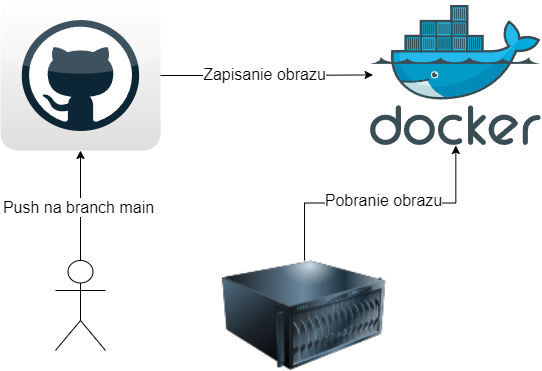
\includegraphics[width=0.7\linewidth]{img/inz_deploy.png}
    \caption{Potok wdrożenia}
    \label{fig:deploy-pipeline}
\end{figure}
Potok wdrożenia jest taki sam dla repozytoriów EMS-API oraz interfejsu użytkownika. Można podzielić go na kolejne etapy, pierwszym z nich jest push'owanie nowej wersji kodu na główny branch repozytorium przez programistę, następnie za pomocą github actions są wykonywane kolejne operacje: testowanie w przypadku EMS-API, następnie zbudowanie obrazu oraz wgranie go do publicznego repozytorium docker-hub. Kolejnym ważnym etapem jest wgranie nowej wersji na produkcję.

\subsubsection{Github actions}
Jest to narzędzie, które nie wymaga dodatkowej konfiguracji czy wdrożenia, jak na przykład Jenkins, ponieważ jest ono wbudowane w github'a. Dzięki temu, w sytuacji, gdy repozytorium jest ulokowane na github'ie, dodanie do niego konkretnych github actions wymaga tylko pojedynczego pliku konfiguracyjnego. W ramach jednego pliku konfiguracyjnego można zdefiniować wiele kroków koniecznych do wykonania. W przykładowym potoku wdrożenia aplikacji EMS-API są 3 takie kroki:
\begin{itemize}
    \item Testowanie
    \item Budowanie obrazu oraz wysłanie go do docker-repository
    \item Wdrożenie produktu na produkcję
\end{itemize}
Każdy z job'ów ma kolejne steps, które są wykonywane w kolejności od góry do dołu. Job'y mogą być wykonywane równolegle, aczkolwiek można definiować między nimi zależności, w tym potoku zależności te wyglądają następująco.
\begin{figure}[H]
    \centering
    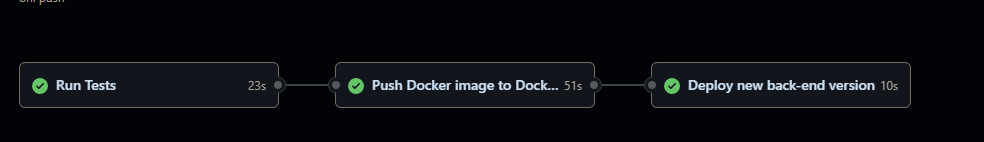
\includegraphics[width=0.75\linewidth]{img/potok-joby.png}
    \caption{Diagram zależności job-ów w potoku}
    \label{fig:jobs-dep}
\end{figure}

Poniżej znajduje się fragment odpowiedzialny za testowanie nowo dodanego kodu - pierwszy job w całym potoku. Ten job wykonuje się zazwyczaj w około 20 sekund.
\begin{minted}{yaml}
run_tests:
name: Run Tests
runs-on: ubuntu-latest
steps:
  - name: Check out the repo
    uses: actions/checkout@v4

  - name: Set up Python
    uses: actions/setup-python@v4
    with:
      python-version: '3.x'
  
  - name: Install dependencies
    run: pip install -r requirements.txt
  
  - name: Run tests
    run: python -m pytest
\end{minted}
Kolejnym etapem jest zbudowanie i wysłanie nowego obrazu do publicznego repozytorium docker'owego, etap ten zajmuje zazwyczaj poniżej minuty. Poniżej znajdują się trzy wybrane fragmenty. W pierwszym możemy zaobserwować, że job ten zależny jest od poprawnego wykonania job'u run\_tests. W kolejnym widać, że z perspektywy actions do docker hub logujemy się za pomocą hasła i loginu umieszczonego w sekretach repozytorium na github. W ostatnim wypychamy gotowy obraz do stworzonego wcześniej repozytorium gambolkf/inz-back.
\begin{minted}{yaml}
name: Push Docker image to Docker Hub
runs-on: ubuntu-latest
needs: run_tests
(...)
  - name: Log in to Docker Hub
    uses: docker/login-action@f4ef78c080cd8ba55a85445d5b36e214a81df20a
    with:
      username: ${{ secrets.DOCKER_USERNAME }}
      password: ${{ secrets.DOCKER_PASSWORD }}
(...)

  - name: Generate artifact attestation
    uses: actions/attest-build-provenance@v1
    with:
      subject-name: docker.io/gambolkf/inz-back
      subject-digest: ${{ steps.push.outputs.digest }}
      push-to-registry: true
\end{minted}
Po wykonaniu tego etapu możemy zaobserwować nowy obraz na docker-hub o nazwie gambolkf/inz-back z tagiem main.

\begin{figure}[H]
    \centering
    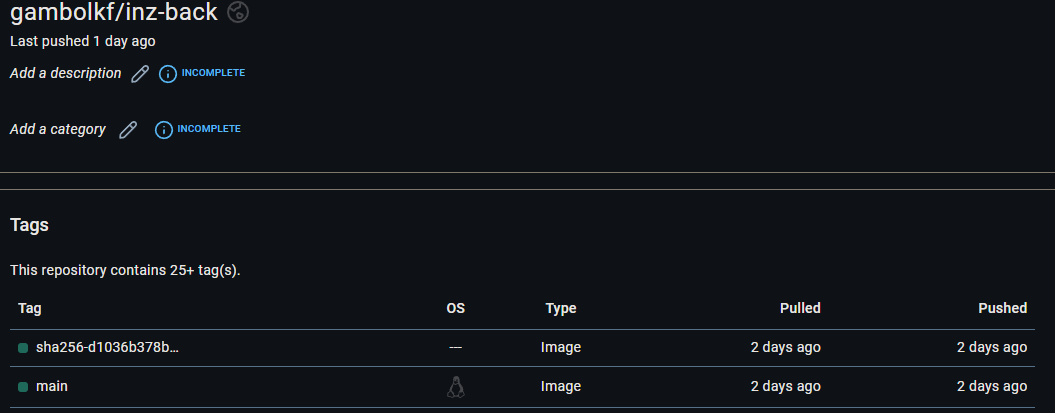
\includegraphics[width=0.75\linewidth]{img/docker-hub-screen.png}
    \caption{Docker-hub obrazy}
    \label{fig:docker0hub-img}
\end{figure}


Ostatnim etapem jest wgranie nowej wersji aplikacji na serwer produkcyjny, odbywa się to za pomocą wywołania komendy Kubernetes'owej- po ssh. Hasło do serwera znajduje się w sekretach github-a.
\begin{minted}{yaml}
deploy_image:
    name: Deploy new back-end version
    runs-on: ubuntu-latest
    needs: push_to_registry
    permissions:
      packages: write
      contents: read
      attestations: write
      id-token: write
    steps:
      - name: Install sshpass
        run: sudo apt-get update && sudo apt-get install -y sshpass

      - name: Restart Deployment on Remote Server
        env:
          SSH_PASSWORD: ${{ secrets.SSH_PASSWORD }}
        run: |
          sshpass -p "$SSH_PASSWORD" ssh -o StrictHostKeyChecking=no kfijalk@49.13.73.66 \
          "minikube kubectl -- rollout restart deployment/fastapi-app -n back"
\end{minted}



\subsection{Stworzenie  odpowiednich abstrakcji Kubernetes'owych}
Aby użyć dockerfile'i w Kubernetes'ie potrzebne jest stworzenie odpowiednich plików konfiguracyjnych. 
\subsubsection{Aplikacje EMS-API, pg\_sync, interfejs użytkownika}
Poniżej znajduje się przykład pliku konfiguracyjnego odpowiadającego za deployment EMS-API. Deployment jest to typ abstrakcji Kubernetes'owej odpowiedzialnej za wdrożenie i zarządzanie pod'ami, ich wersją obrazu, ich ilością, i wieloma innymi elementami. W tym konkretnym Deployment'cie definiujemy jako wersję obrazu obraz: gambolkf/inz-back:main który został wgrany poprzez potok na publiczne repozytorium docker-a. Została również ustawiona flaga imagePullPolicy, dzięki której w momencie restartu tego Deploymentu obraz jest ładowany na nowo. Dzięki takiej konfiguracji za pomocą komendy: `kubectl -- rollout restart deployment/fastapi-app -n back` zostanie wgrana nowa wersja tego deploymentu. Został również wystawiony port 8080 aby był dostęp do API.
\begin{minted}{yaml}
apiVersion: apps/v1
kind: Deployment
metadata:
  name: fastapi-app
  namespace: back
spec:
  replicas: 3
  selector:
    matchLabels:
      app: fastapi-app
  template:
    metadata:
      labels:
        app: fastapi-app
    spec:
      containers:
        - name: fastapi-app
          image: gambolkf/inz-back:main
          imagePullPolicy: Always
          ports:
            - containerPort: 8080
\end{minted}
Kolejną niezbędną abstrakcją jest Kubernetes'owy service. Abstrakcja ta umożliwia komunikację z daną grupą pod'ów za pomocą nazwy serwisu, zamiast np. poszczególnych adresów ip podów. Istnieją różne  typy serwisów, gdzie dla EMS-API najlepszym typem jest NodePort, ponieważ dzięki niemu możemy zdefiniować jaki port jest wystawiony poza sieć Kubernetes'a i po tym porcie komunikować się z danym serwisem z sieci zewnętrznej. Powiązanie między deploymentem a servicem realizowane jest za pomocą sekcji selector, w której zdefiniowane zostało app na tą samą wartość co w deploymencie.
\begin{minted}{yaml}
apiVersion: v1
kind: Service
metadata:
  name: fastapi-app-service
  namespace: back
spec:
  type: NodePort
  ports:
    - port: 80
      targetPort: 8080
      nodePort: 30001
  selector:
    app: fastapi-app
\end{minted}

Dla aplikacji pg\_sync oraz interfejsu użytkownika zarówno deployment jak i service został zdefiniowany analogicznie. Aby pg\_sync mógł działać poprawnie, koniecznie było uruchomienie bazy redis, zostało wykonane to z pomocą helm, następującą komendą:
\begin{minted}{bash}
helm install my-redis bitnami/redis --version 20.3.0
\end{minted}

\subsubsection{Wdrożenie bazy danych Postgres}
Etap ten wykonany jest zgodnie z poradnikiem \cite{DigitalOtionPostgresToK8s}
W celu wdrożenia bazy danych Postgres został również zdefiniowany deployment oraz service. Poza tymi abstrakcjami zostały również wykorzystane: config-map w celu zdefiniowania nazwy bazy, użytkownika oraz hasła. Persistance-Volume zastosowano w celu rezerwacji miejsca na serwerze. Wdrożenie wykonano za pomocą poniższych materiałów:
\begin{minted}{yaml}
apiVersion: v1
kind: PersistentVolume
metadata:
  name: postgres-volume
  labels:
    type: local
    app: postgres
spec:
  storageClassName: manual
  capacity:
    storage: 10Gi
  accessModes:
    - ReadWriteMany
  hostPath:
    path: /data/postgresql
\end{minted}
Zastosowano również persistance-volume claim, które umożliwia korzystanie z danego persistance-volume pod-om
\begin{minted}{yaml}
apiVersion: v1
kind: PersistentVolumeClaim
metadata:
  name: postgres-volume-claim
  labels:
    app: postgres
spec:
  storageClassName: manual
  accessModes:
    - ReadWriteMany
  resources:
    requests:
      storage: 10Gi
\end{minted}

Poza abstrakcjami Kubernetes'owymi, w celu zapewnienia  współpracy bazy z pg\_sync,  wymagane było ustawienie jej dwóch parametrów: wal\_level na logical oraz max\_replication\_slots na więcej niż 1. Wykonane to zostało za pomocą następujących komend wykonanych wewnątrz bazy:
\begin{minted}{bash}
ALTER SYSTEM SET wal_level = logical; ALTER SYSTEM SET max_replication_slots = 5;
\end{minted}
\subsubsection{ELK}
W wykonaniu tego etapu pomocnym był poradnik \cite{ELKTutorial}.
W celu wdrożenia aplikacji monitoringu nazywanych ELK stack, wykorzystany został menadżer pakietów Kubernetes'owych: helm. Zostały pobrane odpowiednie pakiety: elasticsearch, kibana, filebeat, logstash. W większości została przeprowadzona mała edycji plików konfiguracyjnych values.yaml. Dla przykładu, w przypadku pliku konfiguracyjnego elasticsearch edytowane zostały wymagania JVM-a w celu pomniejszenia zapotrzebowania RAM-u. Po edycji, każda z tych aplikacji została zainstalowana za pomocą komendy:
\begin{minted}{bash}
helm install <nazwa aplikacji> <ścieżka do folderu z paczką instalacyjną>
\end{minted}

\subsection{Środowisko produkcyjne}
Jako środowisko produkcyjne wybrany  został serwer na platformie Hetzner. Była to najlepsza forma symulacji środowiska produkcyjnego w najbardziej ekonomicznym rozwiązaniu. Na tym serwerze uruchomiony został klaster Kubernetes'owy za pomocą minikube-a. Jest to narzędzie tworzące mają instancję Kubernetes'a z jednym node-em. Ze uwagi  na tę konkretną konfigurację, zaistniała konieczność dodania narzędzia Ngnix do przekazywania komunikacji na serwer do node-a Kubernetes'owego. Poniżej znajduje się fragment konfiguracji przekazujący komunikację na odpowiedni port node-u.
\begin{minted}{bash}
server {
    listen 80;
    server_name 49.13.73.66;

    location / {
        proxy_pass http://192.168.49.2:30000;
        ...
\end{minted}

Pod adres IP serwera została podpięta również domena. W tym celu wykupiona została domena krzysztof-fij-inz.pl. Jednocześnie na platformie clodflare został zdefiniowany DNS: 
\begin{figure}[H]
    \centering
    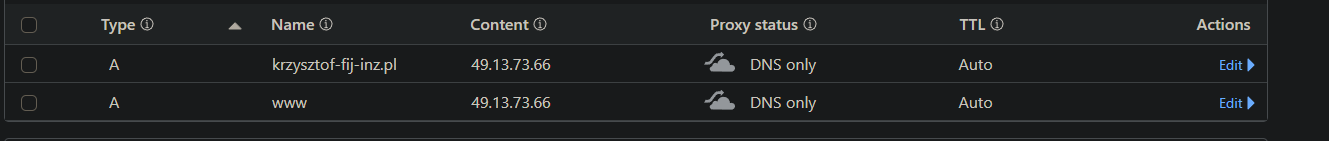
\includegraphics[width=1\linewidth]{img/dns_cloudflare.png}
    \caption{DNS}
    \label{fig:DNS-label}
\end{figure}
Dzięki temu dostęp do serwisu realizowany jest poprzez odwiedzenie domeny krzysztof-fij-inz.pl.
